\documentclass{article}
\usepackage[left=3cm, right=3cm, top=3cm]{geometry}
\usepackage{amsmath}
\usepackage[backend=bibtex,style=verbose-trad2]{biblatex}
\usepackage[T1]{fontenc}
\usepackage{titling}
\usepackage{graphicx}

\setlength{\droptitle}{-10em}
\bibliography{workcited.bib}
\title{Readme File for Github}
\author{Ljuboslav Boskic}
\begin{document}
\maketitle
\section*{Theory}
Koopman operator theory is an alternative formulation of dynamical system theory which provides a versatile framework for data-driven methods of high-dimensional nonlinear systems. The theory originated in the 1930s through the work done by Koopman and Von Neumann \autocite[1]{koopman1932dynamical}. Work done in the previous few years has proven the spectral decomposition\autocite[2]{IM04} \autocite[3]{IM05} , introducing the idea of Koopman modes. This theory led to data-driven methods to approximate the Koopman operator spectrum and modes.\\

In a discrete time setting if:
\begin{equation}
x' = T(x)
\end{equation}
is a discrete time dynamical system where $x\in \mathcal{M}$ and $T: \mathcal{M} \to \mathcal{M}$, the the associated Koopman operator $U$ is defined by:
\begin{equation}
Uf(x)=f\circ T(x)
\end{equation}
We call $\phi: \mathcal{M}\to \mathcal{C}$ an eigenfunction of U associated with $\lambda \in \mathcal{C}$ then,
\begin{equation}
U\phi =\lambda \phi
\end{equation}
And in continous time,
\begin{equation}
U^t\phi = e^{\lambda t}\phi
\end{equation}

The eigenfunctions and eigenvalues of the Koopman operator have lots of information about the dynamics. In the previous years a proof of the Koopman Mode Decomposition (KMD) is another outcome of this theory.\\

The Koopman spectrum consists only of eigenvalues, the evolution of observables can be expanded in terms of Koopman eigenfunction denoted as $\phi_j$ where $(j=0,1...)$ and Koopman eigenvalues $\lambda_j$ where $(j=0,1,...)$.\\
The evolution of $f$ is given by:
\begin{equation}
U^nf(x_o) = f \circ T^n(x_o) = \sum_{j=1}^{\infty} v_j\phi_j(x_o)\lambda_{j}^{n} 
\end{equation}
In this decomposition $v_j$ are the Koopman modes associated with the pair $(\lambda_j,\phi_j)$. These modes correspond to components of the physical field characterized by exponential growth and possible oscillations in time.\\

In recent years, various methods have been made to compute spectral properties $(\lambda,\phi,v)$ from data sets. Data-driven algorithms have been created and utilize data or measurements to approximate the KMD of the system. With this analysis in hand, one is able to identify stability or instability of the modes present within the dynamics. A large fraction of these algorithms are known as Dynamic Mode Decomposition (DMD). 

%% Applications of DMD
\newpage
\section*{Applications of DMD}
The Koopman operator is an infinite-dimensional, linear operator that acts on a Hilbert space of functions called the space of observables. The eigenvalues and eigenfunctions of this linear operator are capable of capturing key dynamics charactersticis of a linear or nonlinear dynamical system. Additionally, the Koopman modes, corresponding to a particular choice of observable function, allow one to reconstruct and forecast (predict) the observed quantity. Togethere these three values of Koopman eigenvalues, eigenfunctions, and modes yield the Koopman mode decomposition (KMD) of an arbitrary observable \autocite[4]{arbabi2017study}. There has been numerous work in control \autocite[5]{arbabi2018data}$^{,}$\autocite[6]{KORDA2018149}\

\subsection*{Temperature Data\autocite[7]{boskic}}
Temperature readings are collected at five locations within a Laboratory at UCSB and an outdoor reading from the Santa Barbara Municipal Airport (\(\sim\) 2 miles away). In addition, there is humidity, light, pressure, and noise measurements for the indoor sensors. Measurements from these sensors (along with outdoor temperature) taken every 5 minutes over the course of 5 days can be found in figure (\ref{SigsFromSens}). Looking at just one sesnor we can see the indoor and outdoor temperature in figure (\ref{SensorInOutMode2l}).
\begin{figure}[!ht]
	\centering
	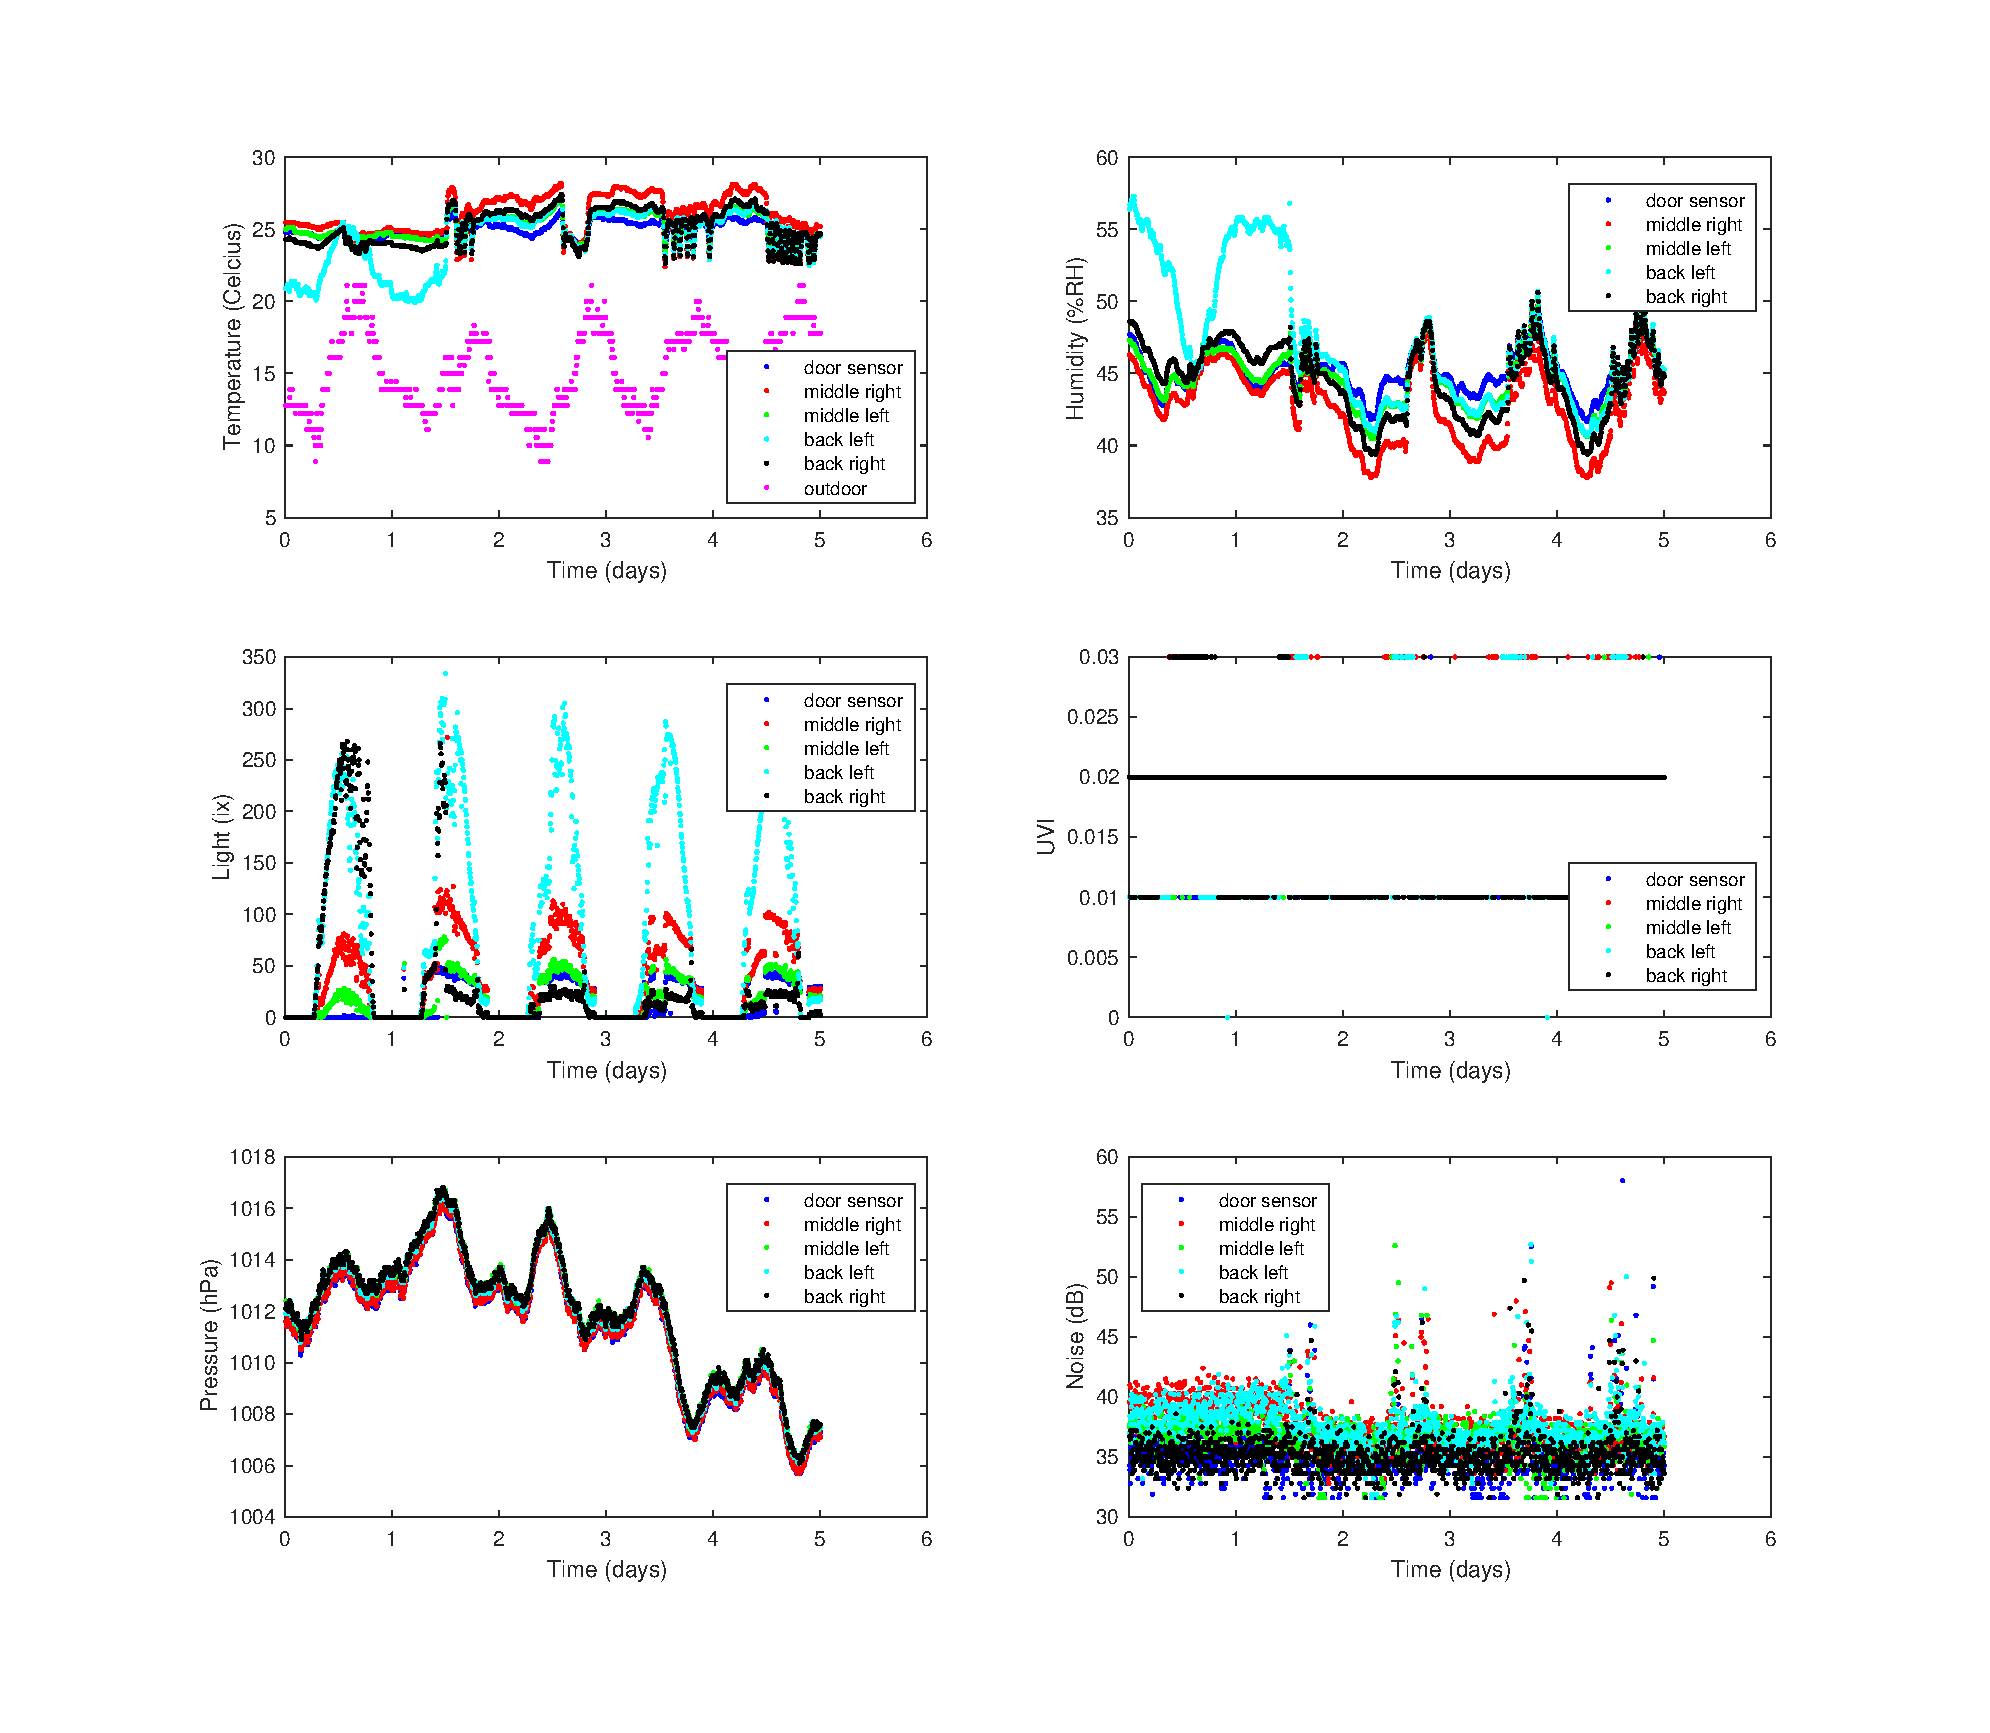
\includegraphics[scale=0.3]{Figures/Signals.pdf}
	\caption{}\label{SigsFromSens}
\end{figure}

\begin{figure} [!ht]
	\centering
	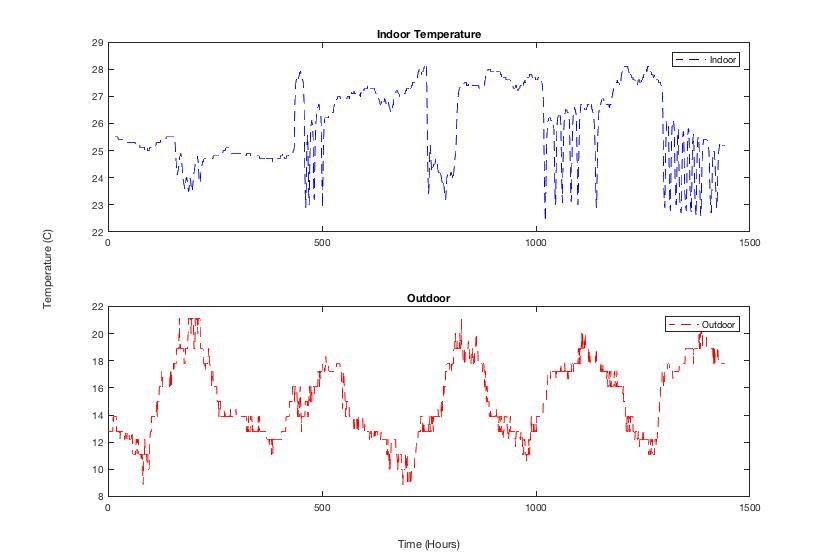
\includegraphics[scale=0.3]{Figures/sensorinout.jpg}
	\caption{Indoor-Outdoor Temperature for May $6^{th}$ 0:00 to May $11^{th}$ 0:00 in laboratory area. This data was taken from the middle right sensor.}
	\label{SensorInOutMode2l}
\end{figure}

In the following figures we have several plots representing Koopman spectral quantities related to our chosen obsevables. In figures (\ref{100D}) and (\ref{200D}) we use 100 and 200, respectively, time shifted observables for each of our six temperature sensors. Both of these figures are structured in the same way:
\begin{enumerate}
\item %%%%
The top left plot contains the frequency of each DMD eigenvalue with its power. Notice the two bumps in the spectrum around a frequency of 15 and 25.
\item %%%%
The top right plot contain the growth rate of each DMD eigenvalue with its power. 
\item %%%%
The second row contains a representation of the first six components of the highest power DMD mode with frequency close to one. The magnitude (left) and complex phase (right) of each of the components of this mode are represented using colors over a simplified diagram of our office.
\item %%%
The third row is similar to the second, but this row represents the highest power mode with frequency near 15. Notice the similarity across changes in observables.

The mode with frequency near one has much larger magnitude for the outside component than for any inside component as we would expect since indoor temperature should be more stable and the outdoor temperature has an obvious one day period. The bumps in the frequency plot near frequencies of 15 and 25 are another consistent feature amongst the plots for different numbers of time-shifted observables. The second DMD mode represented is for the dominant frequency in the first of these bumps. This mode, having a period near 1.5 hours, has much larger components indoor than outdoor, and is related to heating and cooling control. 

The analysis using Koopman modes gives us a remarkable insight into the thermal dynamics of indoor spaces. Namely, the distinction between the zones affected strongly by the outside conditions, near the window, are evident. In addition, there are modes that clearly indicate dynamics of the controllers. In this way, the external influences are separated from control dynamics and the refinement of the analysis using the model in the previous section is possible. {\it For use in residential buildings, such understanding of thermal behavior is of essence in design and control and we have provided the tools for it.}
\end{enumerate}

\begin{figure}[!htbp]
\centering
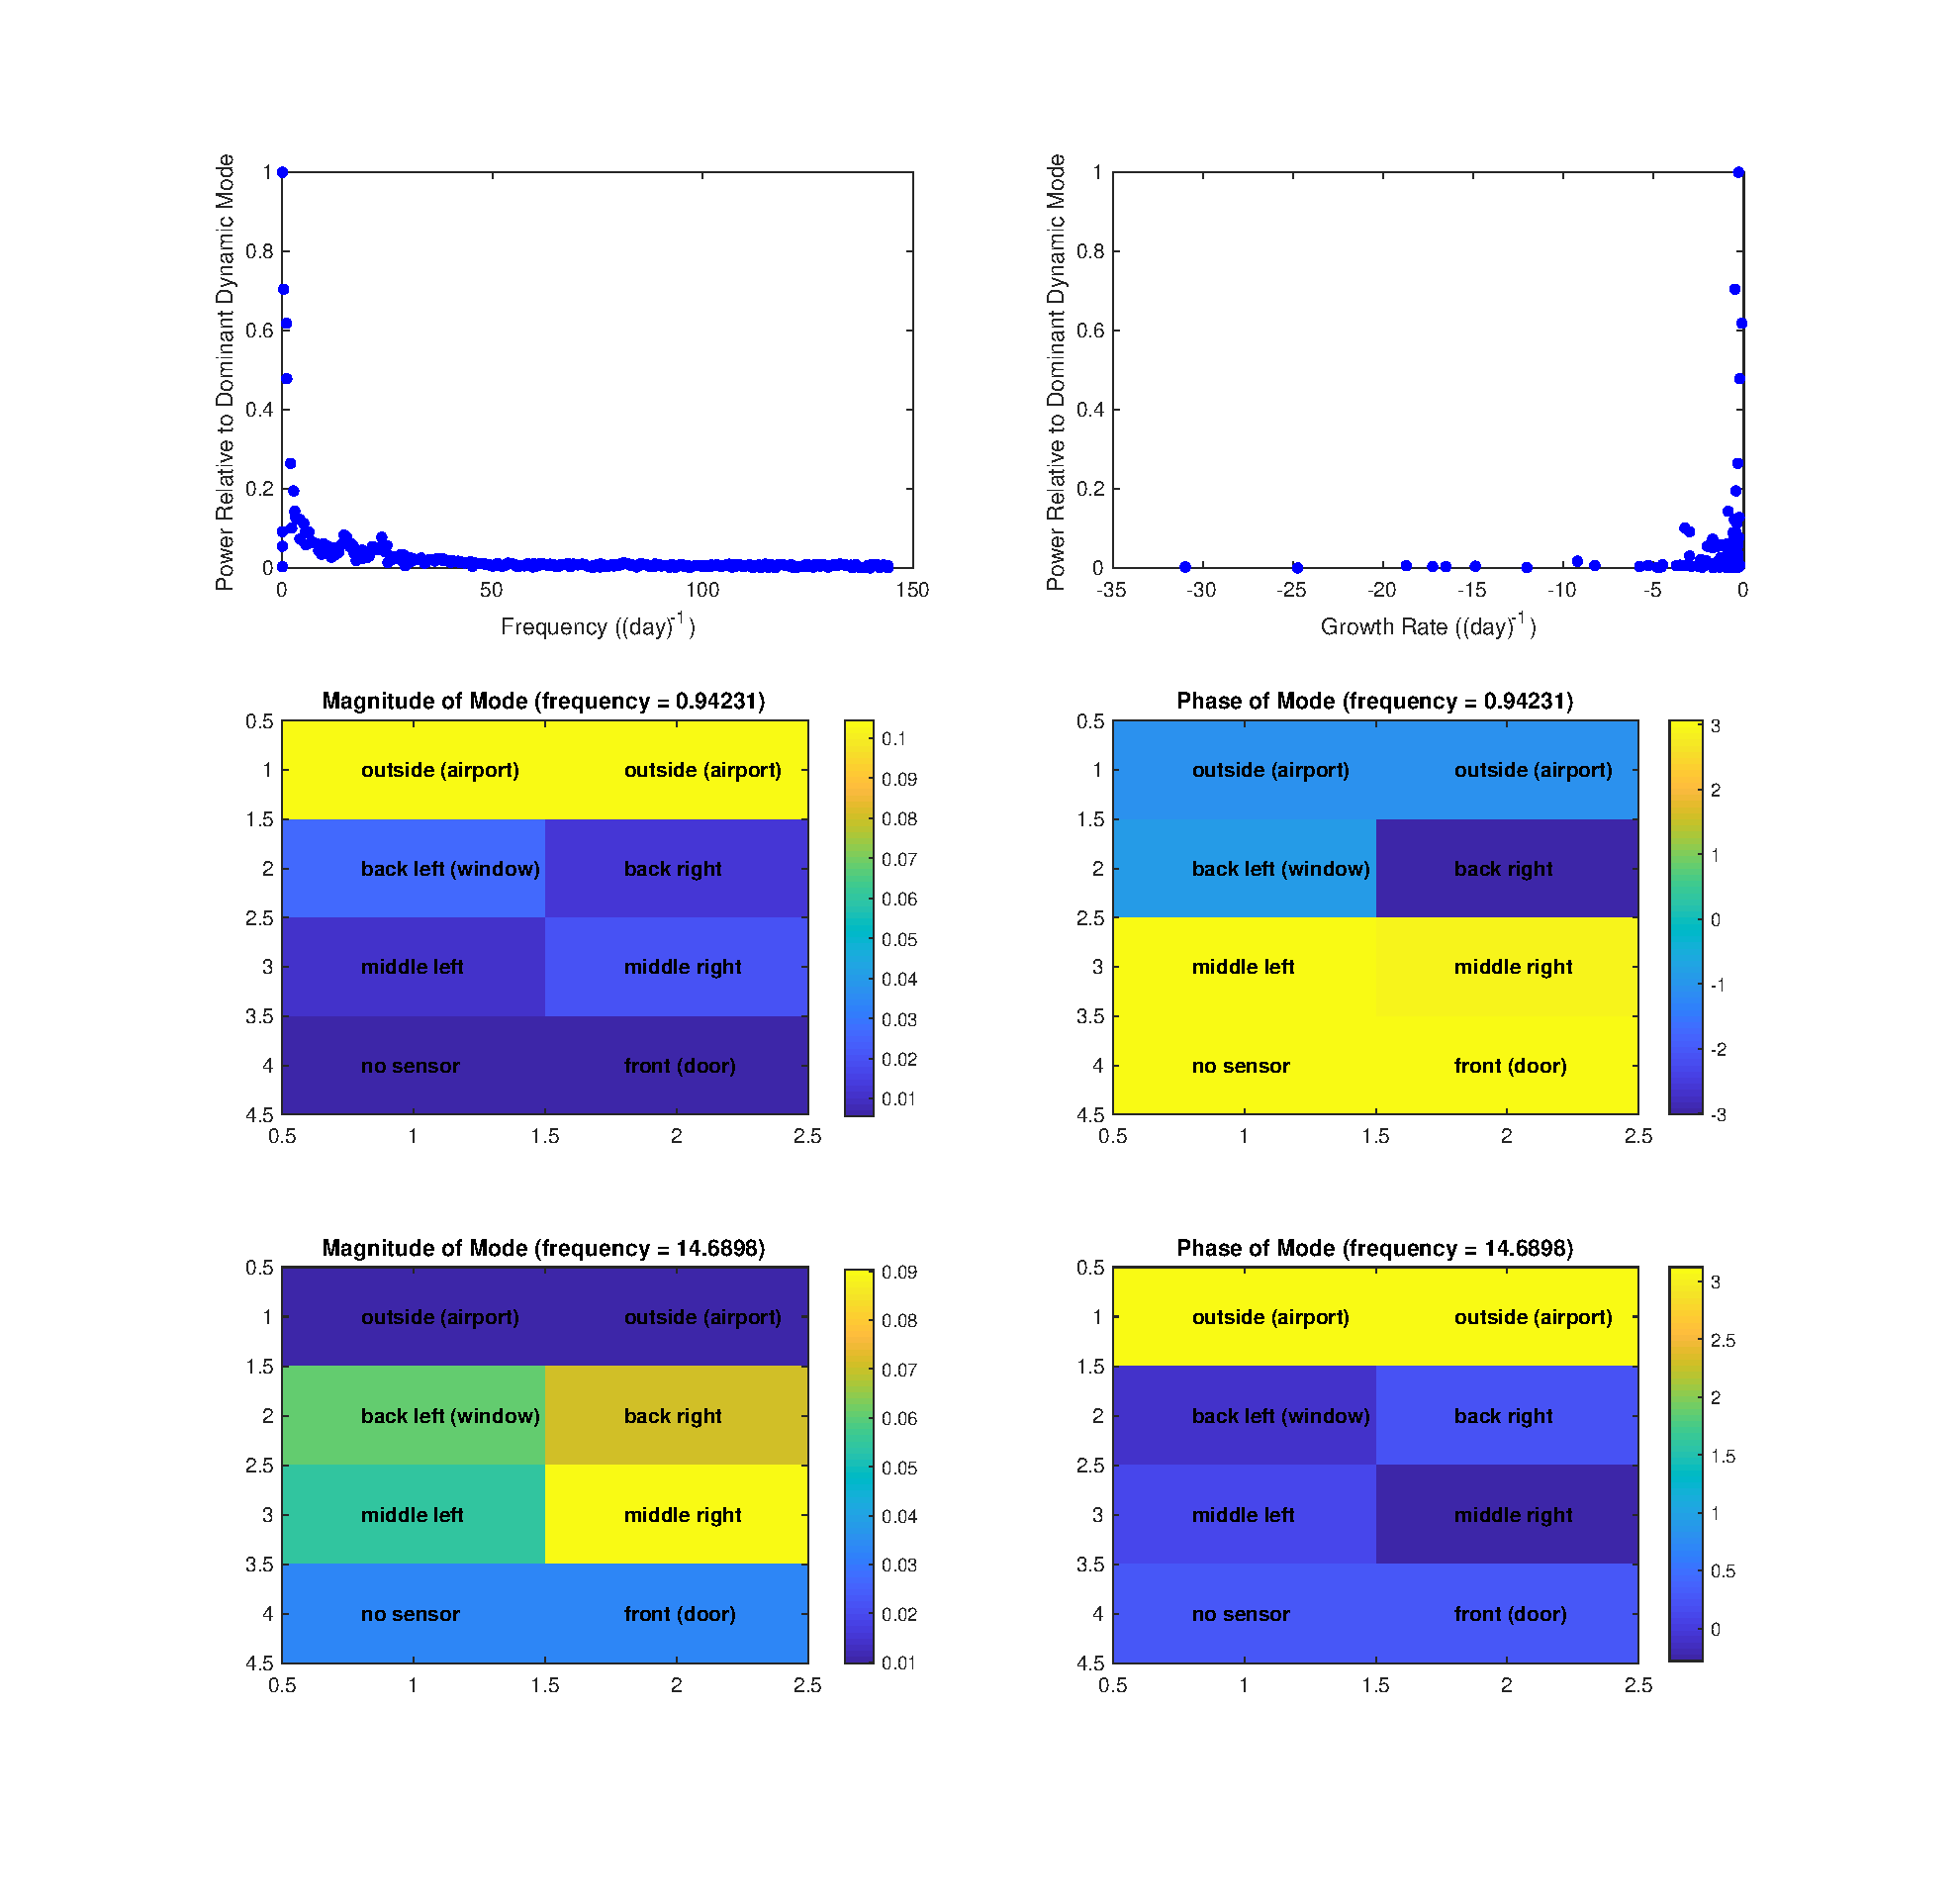
\includegraphics[width=\linewidth]{Figures/100D.pdf}
\caption{}\label{100D}
\end{figure}

\begin{figure}[!htbp]
\centering
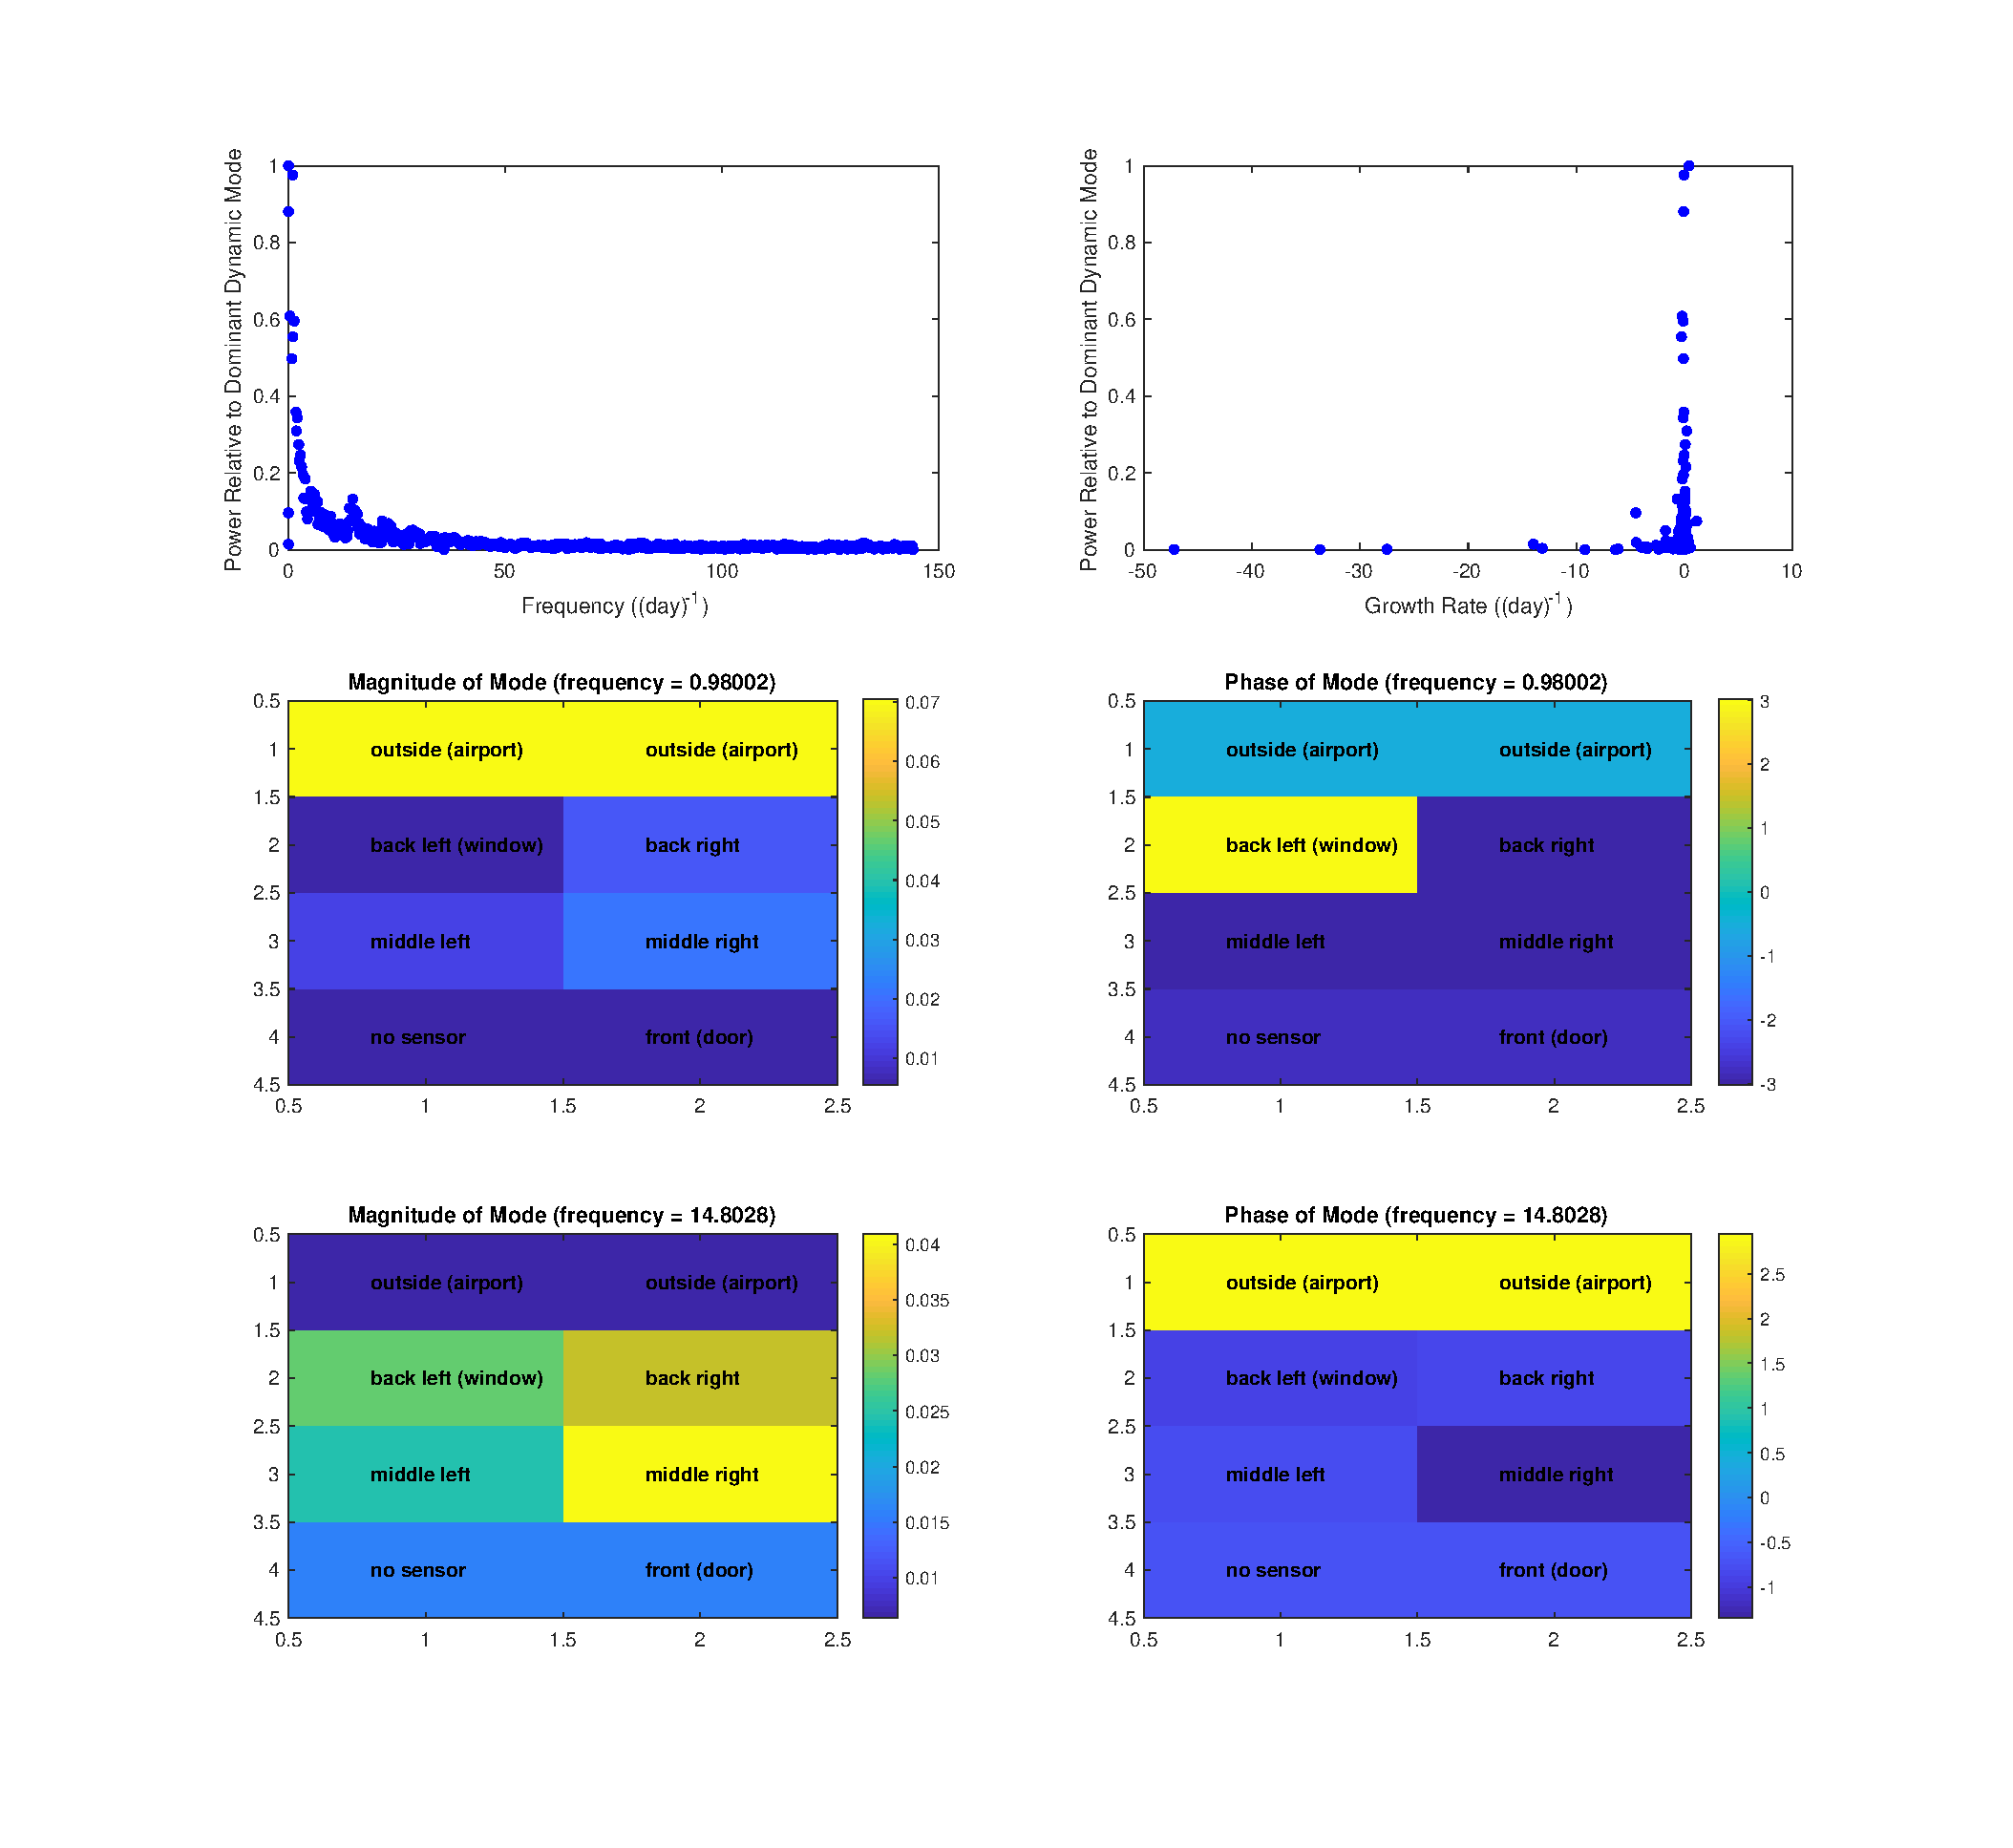
\includegraphics[width=\linewidth]{Figures/200D.pdf}
\caption{}\label{200D}
\end{figure}

%%% Methods
\newpage
\section{Companion Matrix DMD \autocite[8]{YoshiComp}$^{,}$ \autocite[9]{rowley2009spectral}}
We will call $D$ as the data matrix.\\

1) Define $X=[D_o,D_1, \cdots ,D_{m-1}]$\\

2) Compute $c_j$ values:\\
\begin{align*}
X^\dagger D_m = \begin{bmatrix}
c_o \\
c_1 \\
.\\
.\\
.\\
c_{m-2}
\end{bmatrix}
\end{align*}\\
Where $X^\dagger$ is the pseudoinverse of $X$.\\

3) Form the companion matrix:
\begin{align*}
C:= \begin{bmatrix}
0 & 0 &...& 0 &c_o \\
1 &0& ...&  0& c_1 \\
0 &1& ..&. 0& c_2 \\
\vdots& \cdots& \cdots& \cdots & \vdots \\
0 &0& \cdots& 1& c_{m-1}
\end{bmatrix}
\end{align*}\\

4) Get the eigenvalue/vectors from $C$, let $(\lambda_j,w_j)$ be the eigenvalue-vector pair.\\

$\lambda_j$s are the dynamic eigenvalues\

$v_j$s are the dynamic modes\\
\begin{align*}
v_j=Xw_j
\end{align*}

\section{SVD DMD\autocite[10]{tu2013dynamic}}
We will call $D$ as the data matrix.\\

1) Form $X=[D_o,D_1, \cdots ,D_{m-1}]$ and $Y=[D_1,D_2, \cdots,D_m]$\\

2) Compute the singular value decomposition (SVD) of X:
\begin{align*}
svd(X) = U\Sigma V^*
\end{align*}\\

3) Create $\tilde{A}$ matrix:
\begin{align*}
\tilde{A}=U^*YV\Sigma ^{-1}
\end{align*}\\

4) Get the eigenvalue/vectors from $\tilde{A}w=w\lambda$. Let $(\lambda_j,w_j)$ be the eigenvalue-vector pair.\\

$\lambda_j$s are the dynamic eigenvalues\

$v_j$s are the dynamic (projected) modes\\

\begin{align*}
v_j=Uw_j
\end{align*}\\

An alternative eigenvector or Exact DMD Mode $(\phi)$ of $\tilde{A}$ can be given by:
\begin{align*}
v_j = \frac{1}{\lambda_j}(YV\Sigma^{-1}w_j)
\end{align*}

%----- Bibliography ----------------
%\bibliographystyle{unsrt}
%\bibliography{workcited.bib}
%\printbibliography

\end{document}